%\documentclass{sigchi}
\documentclass[chi_draft]{sigchi}

% Load basic packages
\usepackage{balance}       % to better equalize the last page
\usepackage{graphics}      % for EPS, load graphicx instead 
\usepackage[T1]{fontenc}   % for umlauts and other diaeresis
\usepackage{txfonts}
\usepackage{mathptmx}
\usepackage[pdflang={en-US},pdftex]{hyperref}
\usepackage{color}
\usepackage{booktabs}
\usepackage{textcomp}
\usepackage{float}
\usepackage{array}

% Some optional stuff you might like/need.
\usepackage{microtype}        % Improved Tracking and Kerning
% \usepackage[all]{hypcap}    % Fixes bug in hyperref caption linking
\usepackage{ccicons}          % Cite your images correctly!
% \usepackage[utf8]{inputenc} % for a UTF8 editor only

% If you want to use todo notes, marginpars etc. during creation of
% your draft document, you have to enable the "chi_draft" option for
% the document class. To do this, change the very first line to:
% "\documentclass[chi_draft]{sigchi}". You can then place todo notes
% by using the "\todo{...}"  command. Make sure to disable the draft
% option again before submitting your final document.
\usepackage{todonotes}
\usepackage{algorithmicx}
\usepackage{algpseudocode}
\usepackage{algorithm}

% Paper metadata (use plain text, for PDF inclusion and later
% re-using, if desired).  Use \emtpyauthor when submitting for review
% so you remain anonymous.
\def\plaintitle{SIGCHI Conference Proceedings Format}
\def\plainauthor{First Author, Second Author, Third Author,
  Fourth Author, Fifth Author, Sixth Author}
\def\emptyauthor{}
\def\plainkeywords{Authors' choice; of terms; separated; by
  semicolons; include commas, within terms only; required.}
\def\plaingeneralterms{Documentation, Standardization}

% llt: Define a global style for URLs, rather that the default one
\makeatletter
\def\url@leostyle{%
  \@ifundefined{selectfont}{
    \def\UrlFont{\sf}
  }{
    \def\UrlFont{\small\bf\ttfamily}
  }}
\makeatother
\urlstyle{leo}

% To make various LaTeX processors do the right thing with page size.
\def\pprw{8.5in}
\def\pprh{11in}
\special{papersize=\pprw,\pprh}
\setlength{\paperwidth}{\pprw}
\setlength{\paperheight}{\pprh}
\setlength{\pdfpagewidth}{\pprw}
\setlength{\pdfpageheight}{\pprh}

% Make sure hyperref comes last of your loaded packages, to give it a
% fighting chance of not being over-written, since its job is to
% redefine many LaTeX commands.
\definecolor{linkColor}{RGB}{6,125,233}
\hypersetup{%
  pdftitle={\plaintitle},
% Use \plainauthor for final version.
%  pdfauthor={\plainauthor},
  pdfauthor={\emptyauthor},
  pdfkeywords={\plainkeywords},
  pdfdisplaydoctitle=true, % For Accessibility
  bookmarksnumbered,
  pdfstartview={FitH},
  colorlinks,
  citecolor=black,
  filecolor=black,
  linkcolor=black,
  urlcolor=linkColor,
  breaklinks=true,
  hypertexnames=false
}

\def\fluentmotion{\textit{FluentMotion}}
\def\rx{Reactive Extensions}
\def\unity{Unity Game Engine}
\def\leap{LeapMotion}
\def\vr{Virtual Reality}
\def\steamvr{SteamVR}
\def\vive{HTC Vive}
\def\oculus{Oculus Rift}
\def\reactiveui{\textit{ReactiveUI}}

\begin{document}

\pagenumbering{arabic}

\title{FluentMotion - Gesture-based Interaction in Virtual Reality using LeapMotion and Reactive Programming}

\numberofauthors{2}
\author{
  \alignauthor{Radu Petrisel\\
    \affaddr{Technical University of Cluj-Napoca}\\
    \affaddr{28, G. Baritiu Street, 400027} \\
    \affaddr{Cluj-Napoca, Romania}\\
    \email{radupetrisel@gmail.com}}\\
  \alignauthor{Adrian Sabou\\
    \affaddr{Technical University of Cluj-Napoca}\\
    \affaddr{28, G. Baritiu Street, 400027} \\
    \affaddr{Cluj-Napoca, Romania}\\
    \email{adrian.sabou@cs.utcluj.ro}}\\
}

\maketitle

\begin{abstract}
  This paper presents an approach to creating a human readable, flexible and extendable API for gesture-based interaction in Virtual Reality using the \leap{} controller. The \fluentmotion{} API integrates a variety of modern technologies, such as C\# LINQ (Language Integrated Query), \rx{} and \steamvr{}. \fluentmotion{} comes as an extension of the basic \leap{} API, meant to facilitate the integration of gesture-based interaction in Virtual Reality projects. The API integrates with the \unity{}, which provides the means of creating cross-platform \vr{} applications, allowing the definition of new, custom gestures using a human readable description (based on already existing ones) and creating interaction callbacks. \fluentmotion{} works on \vive{} and \oculus{} for VR-enabled application and can also be used in desktop mode. This work improves the rudimentary API offered by \leap{} and offers a more natural, powerful and flexible way of detecting and composing hand and finger gestures.
\end{abstract}

\keywords{Gesture detection; Leap Motion; Virtual Reality; Unity; Reactive Extensions;}

\category{H.5.m.}{Information Interfaces and Presentation} {Human-Computer Interaction} ; {Interaction Techniques} ; {Gestural Input}

\section{General terms}
Virtual Reality; Gesture detection; API

\section{Introduction}
The concept of \vr{} (VR) has been around since the late 20th century, with many prototypes being developed as early as the 1960s. In 2016, the first two consumer headsets were released by HTC and Oculus. Since then, the \vr{} industry grew exponentially, being used in a variety of applications ranging from entertainment to space exploration.

One of the main shortcomings of the current virtual reality setups is the interaction through handheld controllers, which, to many, feels unnatural and unintuitive to use. To solve this issue, LeapMotion released Orion \cite{Orion} in 2016 for its already existing LeapMotion Controller. The controller is a USB device meant to capture hand and finger motions without actually touching it. \leap{}'s basic API for Unity is straightforward, extensible and very well integrated with the game engine, but it lacks flexibility, complex compositions and natural, human-readable description. Thus, the need for a more advanced API arised and \fluentmotion{} was researched and developed with this need in mind.

\fluentmotion{} is an extension of the \leap{} API, based on \rx{} \cite{rx}, meant to facilitate the integration of gesture-based interaction in VR applications, that offers a more natural, powerful and flexible way of detecting and composing hand and finger gestures. \rx{} is an implementation of the observer and iterator design patterns \cite{DPEROOS}, available in many popular languages, such as C\#, Java, C++ and Swift. \rx{} use functional programming in order to reduce the amount of boilerplate code one has to write. The API was partially inspired from \reactiveui{} \cite{ReactiveUI}, a .NET framework for model-view-viewmodel (MVVM) applications based on \rx{}. Some of the gesture detectors' syntax is based on the one of \reactiveui{}'s \textit{ReactiveObject}.

\fluentmotion{} was built for the \unity{}, a very popular game engine, used to empower a large number of VR projects. This provides increased usability, as it can be easily downloaded and integrated in any Untiy project straight from the built-in Unity Package Manager. The user simply adds the \leap{} "prefab" to his project, then builds the \fluentmotion{} hands rig on the \leap{} one. On the new rig, the user can add any gestures (as Unity scripts) to be detected for the hand the script is attached to. Base gestures are defined in abstract classes that must be extended. Only one method needs to be implemented, namely the \textit{OnDetect} callback. Once this is done, the detector is ready for usage.

A custom made application serves as a testbed for the \fluentmotion{} API. The application features a set of icons representing one of the eight tested custom gestures the user has to perform. The icons dynamically change as the gestures are performed and correctly recognized.

The main limitations identified are mainly the ones that affect the \leap{} controller, namely that hand gestures  can only be recognized when performed in the user's field of view. However, one of the shortcomings of the API is the detection of complex moving gestures, which proves difficult. As of the current implementation, the only moving gestures supported are simple swipes.

\section{RELATED WORKS}

Ever since it was introduced to the public, \leap{} promised to offer that which no other controller could do, namely provide natural, gesture-based interaction in VR environments. Even with studies that concluded that \leap{} was not yet suited to compete with traditional input devices in desktop environments, for example as a contact-free pointing device \cite{3149}, in VR it was quickly adopted as a much waited alternative to traditional, unnatural and obtrusive handheld controllers and thus \leap{} enabled VR applications began to appear in the scientific world. Most attempts at using the \leap{} controller in VR either implement the full gesture recognition logic based on a complex, low-level composition and detection API \cite{LMAPI}, or use the complex gesture composition mechanism developed for Unity \cite{LMUAPI}, involving basic detectors and logic gates. 

Kerefeyn and Maleshkov \cite{Kerefeyn} used \leap{} to control and manipulate objects in a VR scenario. Their solution splits the VR logic and the interaction logic and, while the overall interaction style proved to be a success, programming the interaction logic was cumbersome and strictly hard-coded for their application.

Vaitkevi\v{c}ius et al. \cite{Vaitkevicius} used \leap{} to recognize the American Sign Language, building a system that is capable of learning gestures. The detection logic is implemented through the low-level API provided by the controller, extracting four types of hand features and manually composing either stationary or motion enabled gestures.

Khundam \cite{Khundam} use \leap{} to control the movement of a first-person avatar in a VR scene. Movement is controlled by predefined gestures through \leap{}'s SDK for Unity, detected through complex composition of basic detectors using logic gates. The same gesture composition and detection approach is employed by Pop and Sabou in their work on dynamic data visualization and manipulation in VR \cite{Pop}.

While excellent results were obtained in all cases from integrating \leap{} in various VR research, the process of complex gesture composition and detection is encumbering, both through the low-level API and the \leap{} SDK for Unity, the resulting programming logic being restricted to specific use-cases, difficult to extend and, most importantly, difficult to understand by other programmers. As far as we are aware, no other high-level libraries exist that implement the \leap{} gesture recognition logic in a natural, powerful and flexible way, although various hints at possible such ways for structuring such APIs have been identified \cite{zuhlke}.

\section{THE LEAPMOTION CONTROLLER}

\begin{figure}[b]
\centering
  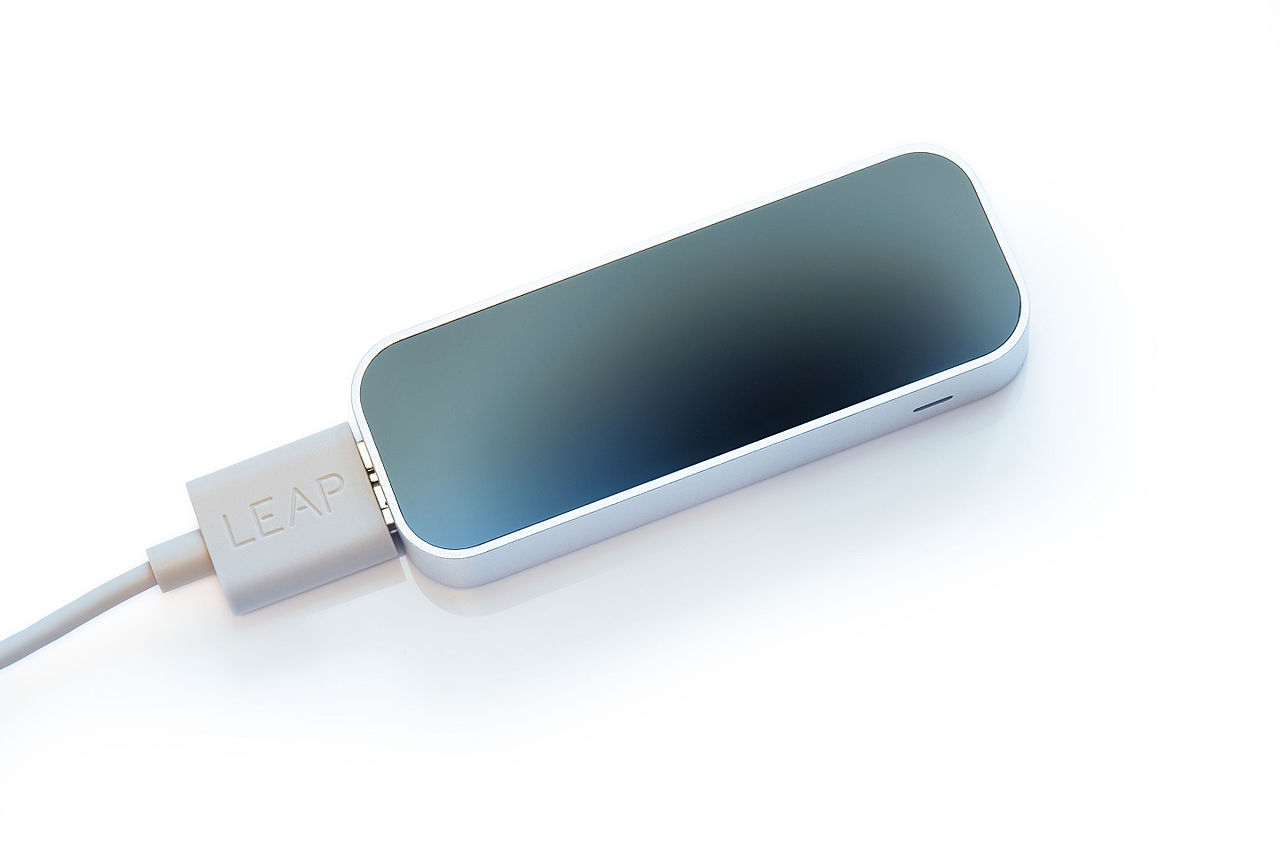
\includegraphics[width=0.9\columnwidth]{figures/LeapMotion_controller}
  \caption{The leapmotion controller}~\label{fig:figure1}
\end{figure}

The \leap{} controller is a device that consists of two stereo cameras which track infrared light with a wavelength of 850 nanometers (allowing it to work even in dark rooms) \cite{LeapArticle}.


The device has a large interaction space, about 0.37 $m^3$. Its range is limited by LED light propagation through space, which is roughly 60cm from the sensor \cite{LeapArticle}.


After the hardware does its job of recording the images, the software starts doing some heavy mathematical lifting. Despite what most users think, the \leap{} controller uses raw sensor data for tracking, not depth maps.


The \leap{} service is responsible for processing this sensor data. Every application that uses \leap{} has a reference to an implementation of this service, either for \vr or for desktop mode. First, the service removes background objects and compensates for ambient lightning, and then reconstructs a 3D representation of the raw device data.


The tracking layer then extracts information from the 3D representation and feeds these results as frames to a transport protocol. From thereon, each application uses this frames as input.


On June 11, 2018, \leap{} released the latest generation of Orion - version 4. It has been in beta since, but it came with major improvements over the past iterations of \leap{}'s tracking software. These include:

\begin{itemize}
  \item increased range of the sensor from 60 to 80cm
  \item faster hand initialization
  \item better hand pose stability and reliability
  \item more accurate shape and scale for hands
\end{itemize}

However, the core of the \leap{} API remains the same and, even though it is straightforward, extensible and very well integrated with the Unity game engine, it still lacks flexibility, complex compositions and natural, human-readable description \cite{LMAPI}.

\section{LEAPMOTION GESTURES}

The \leap{} API \cite{LMAPI} defines mappings for four human body parts:\cite{LMAPI}

\begin{itemize}
  \item \textbf{arm} (from elbow to wrist) - has one hand attached
  \item \textbf{hand} - has five fingers attached
  \item \textbf{finger} - has three joints (for attaching objects) and four bones
  \item \textbf{bone}
\end{itemize}

\leap{} offers a variety of gesture detectors already implemented, which can also be combined by the use of a Logic Gate. The logic gate is a higher level detector, combining two or more basic detectors.

As an example, a "thumbs up" gesture would be detected as combination of the following detectors:

\begin{itemize}
  \item Finger Extended Detector - configured to detect a thumb extended and other fingers not extended
    \begin{figure}[h]
      \centering
      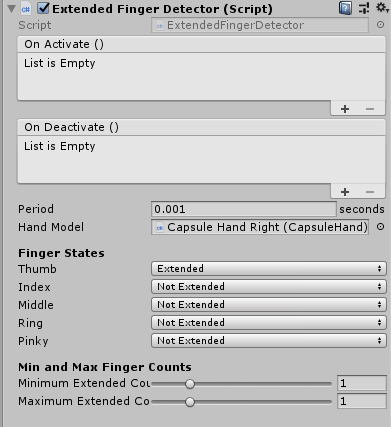
\includegraphics[width=0.7\columnwidth]{figures/ThumbExtendedDetector.png}
      \caption{Leap Thumb extended detector}~\label{fig:figure2}
    \end{figure}
  \item Finger Pointing Detector - configured to detect that the thumb is pointing up (\textit{Vector3(0, 0, 1)}) relative to the horizon
    \begin{figure}[h]
      \centering
      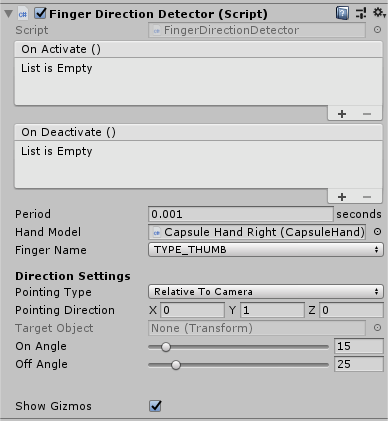
\includegraphics[width=0.7\columnwidth]{figures/ThumbPointingUpDetector.PNG}
      \caption{Leap Thumb pointing up detector}~\label{fig:figure3}
    \end{figure}
  \item And Logic Gate - to combine the other two detectors and have callbacks (C\# scripts) attached to it
    \begin{figure}[h]
      \centering
      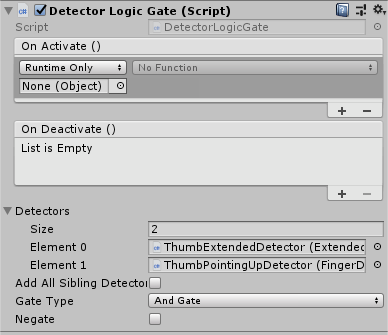
\includegraphics[width=0.7\columnwidth]{figures/ThumbsUpDtector.PNG}
      \caption{Leap Thumb pointing up detector}~\label{fig:figure4}
    \end{figure}
\end{itemize}

This approach requires adding three components to a game object and referencing the first two detectors (Finger Extended Detector and Finger Pointing Detector) from the Logic Gate. This can quickly get out of hand when requiring a high number of combined gestures.

\section{REACTIVE EXTENSIONS}

\begin{figure}[H]
  \centering
  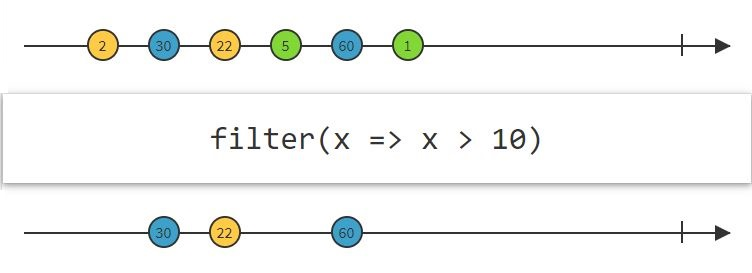
\includegraphics[width=0.9\columnwidth]{figures/RX_filter}
  \caption{Example of a RX operator}~\label{fig:figure5}
\end{figure}
  
ReactiveX is a powerful library for asynchronous and event-based programming. It is an implementation of the observer pattern meant for event-driven programming. It also extends the observer pattern with operators that allow the user to compose sequences declaratively without worrying about low-level concerts (such as mutlithreading and the problems that come with it).


Figure \ref{fig:figure2} shows how an operator works on an observable. In the example, the operator is \textit{filter}. \textit{Filter} takes as input a predicate, a function that maps a value to a boolean (true or false). So, from the source observable [2, 30, 22, 5, 60, 1], by filtering the elemnts greater than 10, we are left with only [30, 22, 60]. Note that the elements are emitted in the same order that they were in the source, almost instantly. The vertical line at the end represents the end of the observable stream. One can attach a callback to that, called \textit{OnComplete}.


The main data structure used by ReactiveX is \textit{Observables}. As stated on their intro page:

\begin{quote}
  You can think of the Observable class as a “push” equivalent to Iterable, which is a “pull.” With an Iterable, the consumer pulls values from the producer and the thread blocks until those values arrive. By contrast, with an Observable the producer pushes values to the consumer whenever values are available. This approach is more flexible, because values can arrive synchronously or asynchronously. (ReactiveX intro)
\end{quote}


The following figures illustrate the resemblance between the iterable and observable.

\begin{algorithm}
  \label{algorithm.iterable}
  \caption{Iterable}
  \begin{algorithmic}
    \State \Call{getDataFromLocalMemory}{$\null$}
      \State .\Call{skip}{10}
      \State .\Call{take}{5}
      \State .\Call{map}{$s \rightarrow s + "transformed"$}
      \State .\Call{forEach}{$println("next \rightarrow" + it)$}
  \end{algorithmic}
\end{algorithm}

% \begin{figure}[h]
%   \centering
%   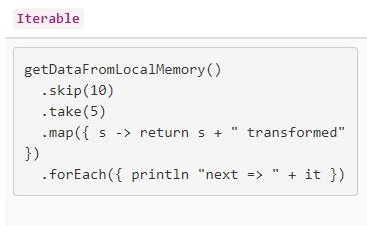
\includegraphics[width=0.9\columnwidth]{figures/RX_iterable}
%   \caption{Iterable}~\label{fig:figure3}
% \end{figure}

\begin{algorithm}
  \label{algorithm.Observable}
  \caption{Iterable}
  \begin{algorithmic}
    \State \Call{getDataFromLocalMemory}{$\null$}
      \State .\Call{skip}{10}
      \State .\Call{take}{5}
      \State .\Call{map}{$s \rightarrow s + "transformed"$}
      \State .\Call{subscribe}{$println("onNext \rightarrow" + it)$}
  \end{algorithmic}
\end{algorithm}

% \begin{figure}[h]
%   \centering
%   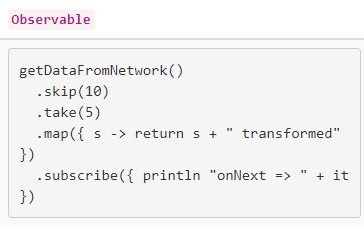
\includegraphics[width=0.9\columnwidth]{figures/RX_observable}
%   \caption{Observable}~\label{fig:figure4}
% \end{figure}

One might say that the only difference is the call to \textit{subscribe} instead of \textit{forEach}. While, indeed, both of the code snippets produce the same result, the real difference is the data flow.


In the \textit{forEach} example, the thread is blocked until 15 elements arrive from the \textit{getDataFromNetwork} call (first 10 are skipped, then only 5 are processed by the \textit{map}).


In the \textit{subscribe} example, the only delay in the thread's execution is the creation of the observable stream, after which other instructions are executed. When data arrives from the \textit{getDataFromNetwork}, the thread which created the observable is interrupted and data is processed.


\section{FLUENTMOTION GESTURES}

From \leap{}'s human body parts, \fluentmotion{} makes use only of \textbf{hands} and \textbf{fingers}, and defines the following basic gestures.

\subsection{Finger Gestures}
\begin{itemize}
  \item \textit{IsExtended} - selected finger is extended
  \item \textit{IsPointingTo} - selected finger is pointing to a given target (Unity Gameobject or a hand)
  \item \textit{AreExtended} - selected fingers are extended (the others are marked as \textit{don't care}, so they could be extended or not)
\end{itemize}

\subsection{Hand Gestures - single hand}

\begin{itemize}
  \item \textit{IsPinching} - hand is pinching (as of Orion 4.4, i.e. \textit{when PinchStrenght > 0.8})
  \item \textit{PalmIsFacing} - palm is facing a given target (can be any object that has a mapping to a Unity \textit{Vector3}) with a given angle tolerance
  \item  \textit{IsFist} - hand is making a fist (i.e. \textit{FistStrenght > 0.8})
  \item \textit{IsMoving} - hand is moving in a given direction (expressed as a Unity \textit{Vector3}) with a given speed (in millimeters per second) and angle tolerance (for the direction) 
\end{itemize}

\subsection{Hand Gestures - both hands}
\begin{itemize}
  \item \textit{PalmsAreFacing} - both palms are facing a target object or, if no object is given, facing each other with a given angle tolerance
  \item \textit{AreMakingFists} - both hands are making fists
  \item \textit{AreMoving} - both hands are moving in a given direction (\textit{Vector3}) and with a given angle tolerance
\end{itemize}

\fluentmotion{} also supports selecting only some fingers from a hand for extra processing, like checking which is extended and which is not or more complex predicates like finger pointing in a dynamically changing direction.


Besides the already defined gestures, users can create their own gesture detectors by implementing the \textit{IReactiveDetector} or by inheriting from one of its three base implementations: \textit{ReactiveFingerDetector}, \textit{ReactiveHandDetector} or \textit{ReactiveHandsDetector}.


The main advantage of \fluentmotion{} is that all gestures - basic and user defined - can be chained indefinitely. Through chaining, more complex gestures can be defined, like swiping right with your left hand while your thumb is up and your index is pointing towards some game object or towards the sky.

\subsection{Unity integration}
After having the \leap{} and \steamvr{} set up, adding \fluentmotion{} to your application is done in two simple steps:

\begin{enumerate}
  \item Add three new empty game objects anywhere in the scene. It is recommended, but not mandatory, to make two of the objects children to the 3\textsuperscript{rd} (as in figure \ref{fig:figure6})
  \begin{figure}[H]
    \centering
    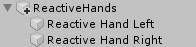
\includegraphics[width=0.9\columnwidth]{figures/FluentMotion_setup}
    \caption{Setting up \fluentmotion{} game objects}~\label{fig:figure6}
  \end{figure}

  \item Attach a \textit{ReactiveHand} script to two of the objects, referencing either the left or the right hand from the LeapRig, and attach a \textit{ReactiveHands} script to the 3\textsuperscript{rd}, referencing the other two \textit{ReactiveHand}s
  \begin{figure}[h]
    \centering
    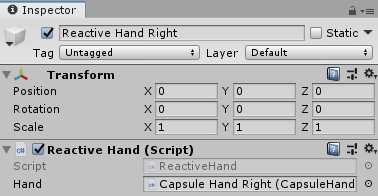
\includegraphics[width=0.9\columnwidth]{figures/FluentMotion_reactive_hand}
    \caption{The \textit{ReactiveHand} script attached to the game object}~\label{fig:figure7}
  \end{figure}
\end{enumerate}

\subsection{Creating Detectors}

To create a detector, extend the \textit{ReactiveHandDetector} class in your own script. As an example, a possible implementation for the "L" gesture - thumb and index are extended, and the others are not - is shows in figure \ref{fig:figure8}.

\begin{figure}[h]
  \centering
  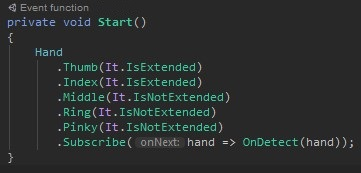
\includegraphics[width=0.9\columnwidth]{figures/FluentMotion_script}
  \caption{The \textit{ReactiveHand} script start function}~\label{fig:figure8}
\end{figure}

The code in figure \ref{fig:figure8} is one of the many ways for expressing this detector. Another option is presented in figure \ref{fig:figure9}.

\begin{figure}[H]
  \centering
  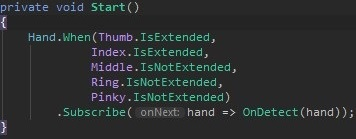
\includegraphics[width=0.9\columnwidth]{figures/FluentMotion_script_alternative}
  \caption{The \textit{ReactiveHand} script start function, using the \textit{When} operator}~\label{fig:figure9}
\end{figure}

The \textit{When} operator is a very powerful construct available in \fluentmotion{}. The first argument to this operator is an optional reduction (combination) lambda function which takes two boolean values as input and returns one boolean value. The default value for this reduction function is the AND operator (the returned boolean value is the logical "and" between the two inputs). Then comes a variable number of predicates, lambda expressions that take as input one value (of the same type as the underlying data stream) and return a boolean value. The combination lambda is applied to each of the predicates' outputs, left to right. If one of the values changes the result of the reduction from \textit{true} to \textit{false}, the reduction process stops (due to the \textit{shortcircuit} property of boolean operators) and the whole data stream cancels.


Of course, a mix of the two methods described in figures \ref{fig:figure8} and \ref{fig:figure9} can be used - say, for when you also want the thumb to point upwards.


The next step is to implement the \textit{OnDetect} method. A possible implementation is shown in figure \ref{fig:figure10}.

\begin{figure}[h]
  \centering
  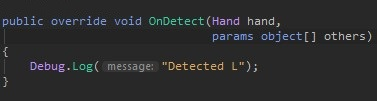
\includegraphics[width=0.9\columnwidth]{figures/FluentMotion_onDetect}
  \caption{\textit{OnDetect} function}~\label{fig:figure10}
\end{figure}

The \textit{params object[] others} are variable arguments - you can pass any extra parameters to this function.


Last, add the script to one of the \textit{ReactiveHand}s in the scene - for example, the right hand - as shown in figure \ref{fig:figure11}. 

\begin{figure}[h]
  \centering
  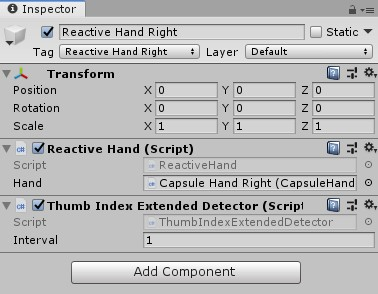
\includegraphics[width=0.9\columnwidth]{figures/FluentMotion_script_attached}
  \caption{Script attached to the right \textit{ReactiveHand}}~\label{fig:figure11}
\end{figure}

The \textit{Interval} field represents the sampling rate expressed in seconds. The sampling rate means how often the same gesture should be detected. The field is of type \textbf{double}, so values less than 1 second can be set. The default value is 500ms (0.5 seconds).

\section{Testing}

For testing purposes, a simple application with 8 possible gestures was created. In the application the is a cube with an icon on it. The icon represents the gesture the cube expects from the player. Once that gesture is detected, the icon (and expected gesture) changes to another random gesture from the pool. The 8 possible gestures and their icon representation are shown in table \ref{tab:table1}.

\begin{table}[h]
  \centering
  \begin{tabular}{ m{5em} m{5em} }
    Gesture & Icon \\
    \hline
    \\
    Thumbs-up & 
\includegraphics[width=0.2\columnwidth]{figures/thumbs-up.png} \\
    "L" & 
\includegraphics[width=0.2\columnwidth]{figures/thumb-index-extended.png} \\
    Fist & 
\includegraphics[width=0.2\columnwidth]{figures/fist.png} \\
    Pinch & 
\includegraphics[width=0.2\columnwidth]{figures/pinch.png} \\ 
    Swipe-up & 
\includegraphics[width=0.2\columnwidth]{figures/swipe-up.png} \\
    Swipe-down & 
\includegraphics[width=0.2\columnwidth]{figures/swipe-down.png} \\
    Swipe-left & 
\includegraphics[width=0.2\columnwidth]{figures/swipe-left.png} \\
    Swipe-right & 
\includegraphics[width=0.2\columnwidth]{figures/swipe-right.png} \\    
  \end{tabular}
  \caption{Gesture to icon mappings}
  \label{tab:table1}
\end{table}

All the gestures are expected to be done by either the left or the right hand. In figure \ref{fig:figure12}, a pinch gesture is made with the right hand, but the cube expects a "L" gesture, so it does nothing.

\begin{figure}[h]
  \centering
  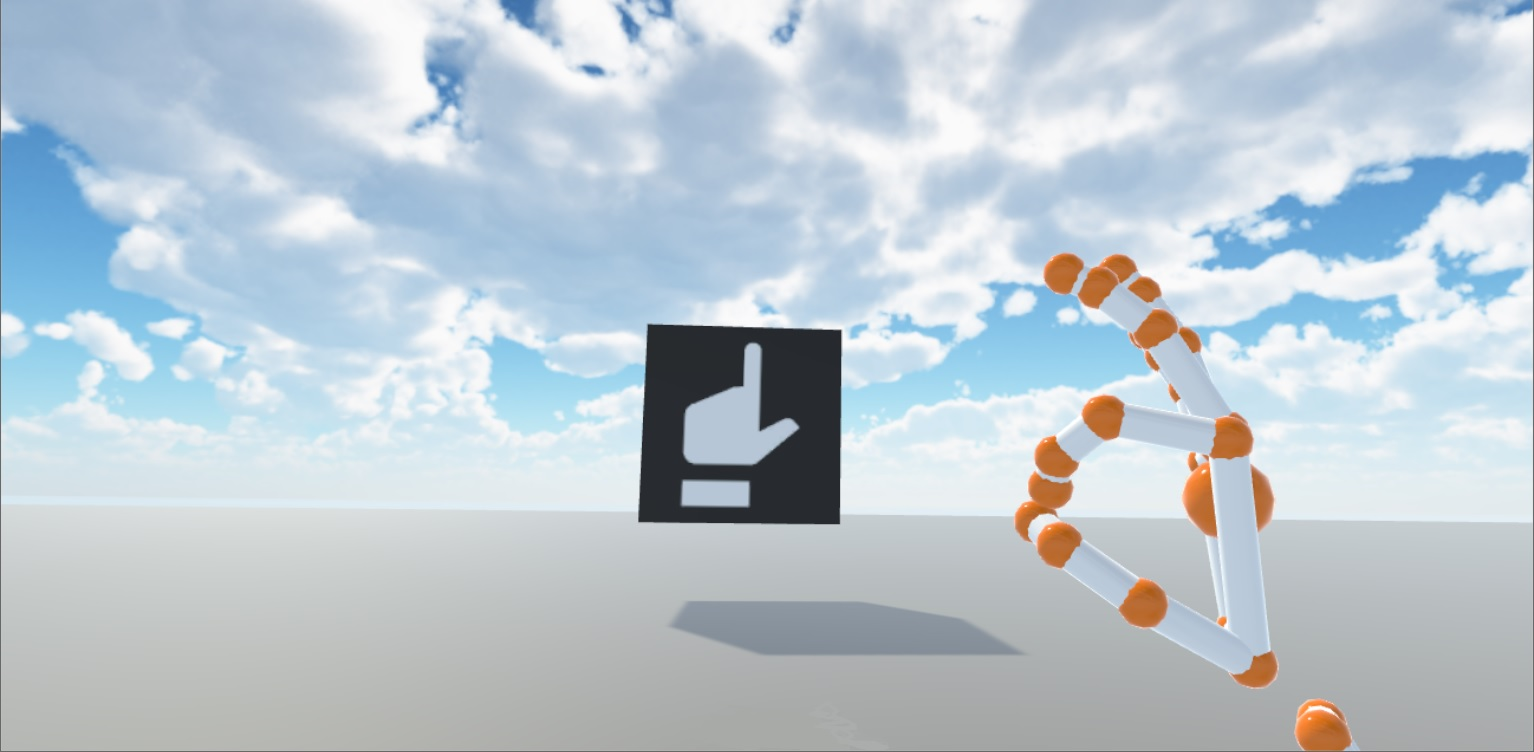
\includegraphics[width=0.9\columnwidth]{figures/Demo_not_detected.jpg}
  \caption{Cube not changing when an incorrect gesture is made}~\label{fig:figure12}
\end{figure}

\section{Performance}

\rx{} operators have varying performance, depending not only on the used operator, but also on the mapping or condition given to that operator. \fluentmotion{} uses only the simpler operators from the RX environment, like \textit{Select, Where, Subscribe} and \textit{Sample}.


Chained operators do not add too big a performance penalty over the simpler ones. This is due to short circuiting in \rx{} operators. That is, if the first operator in a chain fails (the gesture was not detected), all the operators after it aren't hit.


The short circuiting also means that chaining should be done in a careful way. The \textit{IsMoving} operator has a much higher computational cost than the \textit{IsPinching} operator. This means that moving the latter operator higher up the chain greatly impacts the overall performance of the application.


For better performance gains, more than one thread can be used. The user can take advantage of the \rx{}' \textit{ObserveOn(Scheduler.ThereadPool)} operator to schedule a detection chain on a different thread from the RX Pool. 

One minor drawback of the \textit{ObserveOn} is that the thread must be switched back to the main thread before doing any operations on the scene by calling the \textit{ObserveOnMainThread} operator before the \textit{Subscribe} call.

\section{API requirements}

In order to use \fluentmotion{}, the following software requirements exist:

\begin{itemize}
  \item \textbf{Unity Game Engine} 2018.3.7f1 (or newer)
  \item \textbf{UniRX} 6.2.2
  \item \textbf{LeapMotion Orion} 4.0.0
  \item \textbf{LeapMotion Unity Core} 4.4.0
  \item \textbf{LeapMotion Interaction Engine} 1.2.0
  \item \textbf{SteamVR} 2.2.0 
\end{itemize}

Hardware requirements are set by \textbf{SteamVR}, as it is the most demanding of the above mentioned software requirements. Those are:

\begin{itemize}
  \item \textbf{CPU} Intel Core i5Intel Core i5-4590/AMD FX 8350 equivalent or better
  \item \textbf{GPU} NVIDIA GeForce GTX 970, AMD Radeon R9 290 equivalent or better
  \item \textbf{RAM} 4GB
  \item \textbf{VRAM} 4GB
  \item \textbf{OS} Windows 7 SP1, Windows 8.1 or later, Windows 10
\end{itemize}

The hardware requirements apply only to the applications developed using \fluentmotion{}, not to first hand API users (developers).

\section{Conclusions}
\vr{}, even though a new, is a galloping technology whose tendencies are to become closer and closer to the actual reality. This tendency has fueled companies like \leap{} to invent new and more natural means of interacting with the \vr{} world.


Their basic API, though powerful on its own, does not offer much flexibility and readability. This missing features created the need for a new, modern API.

In an attempt to answer this call, \fluentmotion{} could be the needed replacement.

This paper presented the features of this new API, which features a flexible way of defining new gestures, Unity Game Engine integration and increased readability.

Future improvements include continuous gestures (like detecting letters drawn in the air) and the detection of "negated gestures" (\textit{detect when *this* does not occur}).

% BALANCE COLUMNS
\balance{}

\bibliographystyle{SIGCHI-Reference-Format}
\bibliography{FluentMotion}

\end{document}

%%% Local Variables:
%%% mode: latex
%%% TeX-master: t
%%% End:
